%% For double-blind review submission, w/o CCS and ACM Reference (max submission space)
%\documentclass[sigplan,10pt,review,anonymous]{acmart}
%\settopmatter{printfolios=true,printccs=false,printacmref=false}
%% For double-blind review submission, w/ CCS and ACM Reference
%\documentclass[sigplan,review,anonymous]{acmart}\settopmatter{printfolios=true}
%% For single-blind review submission, w/o CCS and ACM Reference (max submission space)
%\documentclass[sigplan,review]{acmart}\settopmatter{printfolios=true,printccs=false,printacmref=false}
%% For single-blind review submission, w/ CCS and ACM Reference
%\documentclass[sigplan,review]{acmart}\settopmatter{printfolios=true}
%% For final camera-ready submission, w/ required CCS and ACM Reference
\documentclass[acmsmall]{acmart}\settopmatter{printccs=false,printacmref=false}


%% Conference information
%% Supplied to authors by publisher for camera-ready submission;
%% use defaults for review submission.
\acmConference{University of Michigan}{April, 2022}{Ann Arbor, MI, USA}
\acmISBN{} % \acmISBN{978-x-xxxx-xxxx-x/YY/MM}
\acmDOI{} % \acmDOI{10.1145/nnnnnnn.nnnnnnn}
\startPage{1}

%% Copyright information
%% Supplied to authors (based on authors' rights management selection;
%% see authors.acm.org) by publisher for camera-ready submission;
%% use 'none' for review submission.
\setcopyright{none}
%\setcopyright{acmcopyright}
%\setcopyright{acmlicensed}
%\setcopyright{rightsretained}
%\copyrightyear{2018}           %% If different from \acmYear

%% Bibliography style
\bibliographystyle{ACM-Reference-Format}
%% Citation style
\citestyle{acmauthoryear}  %% For author/year citations
%\citestyle{acmnumeric}     %% For numeric citations
%\setcitestyle{nosort}      %% With 'acmnumeric', to disable automatic
                            %% sorting of references within a single citation;
                            %% e.g., \cite{Smith99,Carpenter05,Baker12}
                            %% rendered as [14,5,2] rather than [2,5,14].
%\setcitesyle{nocompress}   %% With 'acmnumeric', to disable automatic
                            %% compression of sequential references within a
                            %% single citation;
                            %% e.g., \cite{Baker12,Baker14,Baker16}
                            %% rendered as [2,3,4] rather than [2-4].


%%%%%%%%%%%%%%%%%%%%%%%%%%%%%%%%%%%%%%%%%%%%%%%%%%%%%%%%%%%%%%%%%%%%%%
%% Note: Authors migrating a paper from traditional SIGPLAN
%% proceedings format to PACMPL format must update the
%% '\documentclass' and topmatter commands above; see
%% 'acmart-pacmpl-template.tex'.
%%%%%%%%%%%%%%%%%%%%%%%%%%%%%%%%%%%%%%%%%%%%%%%%%%%%%%%%%%%%%%%%%%%%%%


%% Some recommended packages.
\usepackage{booktabs}   %% For formal tables:
                        %% http://ctan.org/pkg/booktabs
\usepackage{subfig} %% For complex figures with subfigures/subcaptions
                        %% http://ctan.org/pkg/subcaption
\usepackage[export]{adjustbox}

\usepackage[T1]{fontenc} % fix missing font cmtt
\usepackage{amsmath}
\let\Bbbk\relax
\usepackage{amssymb} % Vdash
\usepackage{graphicx} % rotatebox
\usepackage{stmaryrd} % llparenthesis
\usepackage{anyfontsize} % workaround for font size difference warning
\usepackage{todonotes}
\usepackage{listings}
\usepackage{tikz}
\usetikzlibrary{calc,fit,tikzmark,plotmarks,arrows.meta,positioning,overlay-beamer-styles}

\usepackage{cancel} % slash over symbol
\usepackage{hyperref}
\renewcommand\UrlFont{\color{blue}\rmfamily}
\def\figureautorefname{Fig.}
\def\lemmaautorefname{Lemma}
\def\sectionautorefname{Sec.}
\let\subsectionautorefname\sectionautorefname
\let\subsubsectionautorefname\sectionautorefname
\newcommand{\rulesref}[1]{Rules (\ref{#1})}
\newcommand{\ruleref}[1]{Rule (\ref{#1})}

\usepackage{xcolor}
\definecolor{hazelgreen}{RGB}{7,63,36}
\definecolor{hazellightgreen}{RGB}{103,138,97}
\definecolor{hazelyellow}{RGB}{245,222,179}
\definecolor{hazellightyellow}{RGB}{254,254,234}

\newcommand{\highlight}[1]{\colorbox{yellow}{$\displaystyle #1$}}

\usepackage{listings}%
\lstloadlanguages{ML}
\lstset{tabsize=2, 
	basicstyle=\fontsize{7.5pt}{1em}\ttfamily, 
	% keywordstyle=\sffamily,
	commentstyle=\itshape\ttfamily\color{gray}, 
	stringstyle=\ttfamily\color{purple},
	mathescape=false,escapechar=\#,
	numbers=left, numberstyle=\scriptsize\color{gray}\ttfamily, language=ML, showspaces=false,showstringspaces=false,xleftmargin=15pt, 
	morekeywords={string, float, int, bool, match},
	classoffset=0,belowskip=\smallskipamount, aboveskip=\smallskipamount,
	moredelim=**[is][\color{red}]{SSTR}{ESTR}
}
\newcommand{\li}[1]{\lstinline[basicstyle=\ttfamily\fontsize{9pt}{1em}\selectfont]{#1}}
\newcommand{\lismall}[1]{\lstinline[basicstyle=\ttfamily\fontsize{9pt}{1em}\selectfont]{#1}}

\begin{document}

%% Title information
\title{Pattern Matching with Typed Holes}         %% [Short Title] is optional;
                                        %% when present, will be used in
                                        %% header instead of Full Title.
                                        %% contents suppressed with 'anonymous'
\subtitle{Proposal for Computer Science Honors Thesis}                     %% \subtitle is optional
                                        %% can be repeated if necessary;
                                        %% contents suppressed with 'anonymous'


%% Author information
%% Contents and number of authors suppressed with 'anonymous'.
%% Each author should be introduced by \author, followed by
%% \authornote (optional), \orcid (optional), \affiliation, and
%% \email.
%% An author may have multiple affiliations and/or emails; repeat the
%% appropriate command.
%% Many elements are not rendered, but should be provided for metadata
%% extraction tools.

%% Author with single affiliation.
\author{Scott Guest}
\orcid{nnnn-nnnn-nnnn-nnnn}             %% \orcid is optional
\affiliation{
  \institution{University of Michigan}            %% \institution is required
}
\email{sguest@umich.edu}          %% \email is recommended

%% Author with two affiliations and emails.
\author{Cyrus Omar}
\affiliation{
  \institution{University of Michigan}           %% \institution is required
}
\email{comar@umich.edu}         %% \email is recommended


%% Abstract
%% Note: \begin{abstract}...\end{abstract} environment must come
%% before \maketitle command
\begin{abstract}
	To support reasoning about incomplete programs in a principled way, various programming systems have introduced \emph{typed-holes} - placeholder terms which indicate missing syntactic pieces or semantic inconsistencies \cite{GHCHoles, DBLP:journals/jfp/Brady13, DBLP:conf/icfp/Norell13, DBLP:conf/popl/OmarVHAH17}. Ideally, these holes allow every intermediate edit state of a program to be given static or even dynamic meaning, with the aim of enabling simpler and more powerful development tools \cite{DBLP:conf/snapl/OmarVHSGAH17, DBLP:journals/pacmpl/OmarVCH19}. However, current systems are limited in that they only support holes in expressions or types, presenting difficulty when editing binding constructs such as patterns. To resolve this, we have developed Peanut: a calculus for pattern matching with typed pattern holes, including support for exhaustiveness and redundancy checking in this setting. Additionally, we also provide a mechanization of Peanut's semantics and metatheory in the Agda proof-assistant \cite{norell:thesis}.
\end{abstract}
%% End of generated code


%% \maketitle
%% Note: \maketitle command must come after title commands, author
%% commands, abstract environment, Computing Classification System
%% environment and commands, and keywords command.
\maketitle

\section{Introduction}\label{sec:intro}

For the modern programmer, development has progressed beyond the unassisted writing of code in a text editor, and it now increasingly involves conversing with a wide-variety of programming tools. As incremental changes are made, type checkers, debuggers, interpreters, program synthesizers and so forth all provide feedback, seeking to increase programmer productivity or ensure program correctness. Unfortunately, however, programming languages typically only assign meaning to programs which are already fully-formed and well-typed. As a result, these tools struggle to deal with what is perhaps one of the most common states of a program during development: an unfinished piece of work with ongoing, syntax-breaking editing or as-yet-unresolved semantic errors. Throughout the editing process then, feedback from these tools is only available sporadically, limiting their usefulness when they are needed most.

This troublesome issue, where programming tools have gaps in their services throughout the editing process, is aptly known as the \emph{gap problem}. Previously, most attempts to close such gaps have relied on \textit{ad hoc} or fragile heuristics, for example, making assumptions about missing tokens, or ignoring large swathes of invalid code all together \cite{DBLP:conf/oopsla/KatsJNV09, DBLP:conf/snapl/OmarVHSGAH17}. Recently though, the work of  \cite{DBLP:conf/snapl/OmarVHSGAH17} has outlined a more principled approach: rather than treating intermediate edit states as meaningless, one can extend a language's syntax and semantics to explicitly represent all such states as well-formed terms. Every editor state can then be assigned static or even dynamic meaning, allowing programming tools to handle them in a uniform way and removing the need for such \emph{ad hoc} heuristics.

To varying degree, systems including Haskell \cite{GHCHoles}, Idris \cite{DBLP:journals/jfp/Brady13}, Agda \cite{DBLP:conf/icfp/Norell13}, and Hazel \cite{DBLP:conf/popl/OmarVHAH17} implement this approach through a feature known as \emph{typed-holes}. When a program has a missing syntactic piece, rather than treating the entire program as meaningless, we localize the issue by inserting an \emph{empty hole} expression at the unfinished location. Likewise, semantically inconsistent expressions, e.g. those that are ill-typed or reference undefined identifiers, may be wrapped with a \emph{non-empty hole} expression, isolating the inconsistency from the program at large. Tools can then the aid the developer by providing static information about these holes - displaying the variables and types in scope, inferring the expected type, or even synthesizing possible hole-fillings \cite{DBLP:conf/haskell/Gissurarson18, DBLP:journals/pacmpl/LubinCOC20}. 

\begin{figure}
	\centering
	\subcaptionbox{Empty and non-empty holes\label{fig:arith-initial}}{
		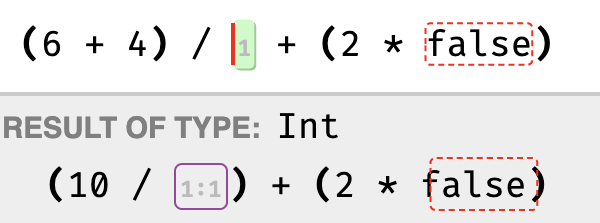
\includegraphics[scale=0.47,valign=t]{imgs/arith-initial.png}%
		\vphantom{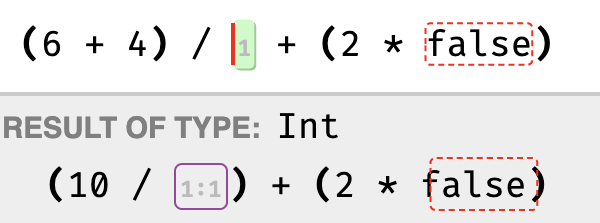
\includegraphics[scale=0.47,valign=t]{imgs/arith-initial.png}}
	}
	\hfil
	\subcaptionbox{Result after filling empty hole\label{fig:arith-partial}}{
		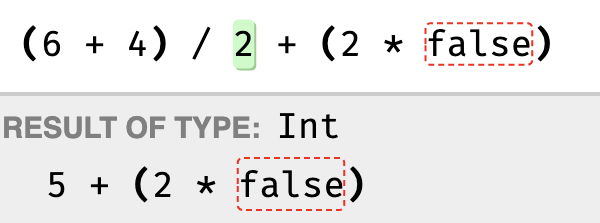
\includegraphics[scale=0.47,valign=t]{imgs/arith-partial.png}%
	 	\vphantom{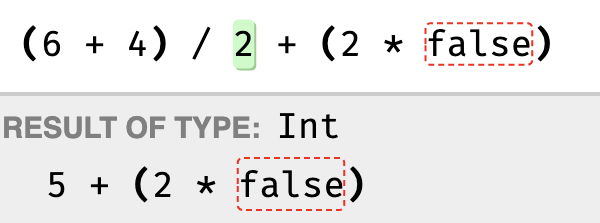
\includegraphics[scale=0.47,valign=t]{imgs/arith-partial.png}}
	}
	\hfil\par\bigskip
	\subcaptionbox{Result after filling non-empty hole\label{fig:arith-complete}}{
		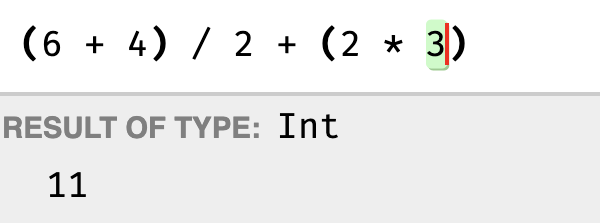
\includegraphics[scale=0.47,valign=t]{imgs/arith-complete.png}
	}
	\caption{Live Evaluation with Expression Holes}
	\label{fig:arith-example}
\end{figure}

Most notable among the aforementioned systems is Hazel - a structure editor which was designed from logical and type-theoretic first principles to seamlessly and fully-automatically insert holes throughout the editing process. Starting from an empty hole, every possible program can be built up using a set of edit actions which directly manipulate the syntax tree. Along the way, Hazel maintains a \emph{maximal liveness} invariant so that every intermediate step is a valid term with well-defined static and dynamic semantics, completely eliminating the gap problem \cite{DBLP:journals/pacmpl/OmarVCH19}. \autoref{fig:arith-example} displays screenshots of a small part of the Hazel editor, with the user in the process of editing a simple arithmetic expression. Considering only Fig.~\ref{fig:arith-initial} for now, both variants of typed-holes are present: an empty hole labeled with id \li{1} indicates a missing piece of the expression, and a non-empty hole, shown as a dashed red box, serves as a membrane around the type inconsistency related to the term \li{false}.

One of  Hazel's main contributions is its comprehensive dynamic semantics which allows evaluation to continue "around holes", thereby preventing gaps in services which rely on actual program execution \cite{DBLP:journals/pacmpl/OmarVCH19}. This stands in contrast to systems such as Haskell, which, when supplied with appropriate compiler flags, treat holes as panics - reminiscent of a common pattern where developers raise an exception at yet-to-be-implemented code locations \cite{GHCHoles}. With Hazel, however, upon evaluation encountering a hole, rather than panicking or otherwise terminating the program, Hazel defers the evaluation of that particular expression and those that rely on. It then continues to evaluate all other complete (i.e. hole-less) parts of the program until no such evaluation is possible. Finally, evaluation pauses, yielding an \emph{indeterminate} value if there are still holes present. At a later time, the remaining holes in this indeterminate result can be filled, and evaluation resumes without having to restart the program. As a result, Hazel provides continuous live feedback throughout the entire editing process.

The rest of \autoref{fig:arith-example} demonstrates this live evaluation. Initially, the expression shown in Fig.~\ref{fig:arith-initial} contains two holes. Hazel partially evaluates the expression, reducing the complete term \li{6 + 4} to \li{10}, but can perform no further reductions. An indeterminate result is displayed, still containing both holes present in the initial expression. In Fig.~\ref{fig:arith-partial}, we then fill the empty hole with id \li{1} using the value \li{2}. This allows evaluation to resume, further reducing \li{(6 + 4) / 2} to \li{5}, but again pausing due to the presence of the non-empty hole. Finally, in Fig.~\ref{fig:arith-complete}, we resolve the typing inconsistency by replacing the term \li{false} with the integer \li{3}. The non-empty hole is automatically removed, and Hazel now produces a concrete value \li{11}. At no point during this process is the editor state meaningless, nor is the program ever restarted.

While Hazel itself is still under development, and is currently little more than a lambda calculus with primitive types, sums, and products, it seeks to soon reach feature-parity with production-level languages such as Elm \cite{DBLP:conf/pldi/CzaplickiC13, Elm, DBLP:journals/pacmpl/OmarVCH19}. Indeed, the machinery behind Hazel is not limited to its specific features, but rather, it provides a systematic, near-mechanical way to build similar structure editors for any language. Its semantics are built up using common techniques from gradual typing \cite{DBLP:conf/snapl/SiekVCB15}: holes are considered to have the unknown type, and terms are elaborated into a cast calculus to handle such typing at runtime. Additional machinery from contextual modal type theory \cite{DBLP:journals/tocl/NanevskiPP08} is then used to track substitutions which occur around holes, allowing holes to be filled in any order while producing the same final result. Given this principled theoretical basis, future work may even allow us to algorithmically generate Hazel-like structure editors for numerous languages in a fully automatic way, developing something akin to the Gradualizer \cite{DBLP:conf/popl/CiminiS16}. However, for any of this development be possible, and indeed to apply Hazel's techniques to any full-fledged functional programming language at all, one commonplace feature still needs more careful consideration: \emph{structural pattern matching}.

Throughout the rest of this paper, we tackle the challenge of integrating pattern matching into a Hazel-like system while seeking to maintain the maximal liveness invariant. We begin in \autoref{sec:background} by reviewing the required background and terminology for pattern matching in general. In \autoref{sec:pattern-matching}, we then introduce the concept of a \emph{pattern hole}, and provide a high-level discussion of our desired semantics for pattern matching with these holes, including redundancy and exhaustiveness in this setting. Finally,  in \autoref{sec:peanut}, we formalize this high-level discussion, presenting our work as a type theoretic calculus Peanut which extends the Hazelnut Live internal language 
of \cite{DBLP:journals/pacmpl/OmarVCH19}. To round off the development, we also outline algorithmic implementations of redundancy and exhaustiveness checking in \autoref{sec:decidability}, then discuss an Agda mechanization of Peanut's semantics and metatheory in \autoref{sec:mechanization}.

\section{Pattern Matching with Typed Holes in Hazel}\label{sec:pattern-matching}

Let us now return to the problem of extending Hazel with pattern matching, placing particular emphasis on maintaining Hazel's maximal liveness invariant. Presently, all current systems with typed-holes only support holes in expressions or types, but notably, do not permit holes in binding constructs such as patterns. As a result, when editing a pattern - a necessarily incremental process - a user still faces meaningless editor states and thus gaps in editor services. To resolve this, we again turn to the approach outlined in \cite{DBLP:conf/snapl/OmarVHSGAH17}, extending our language to represent such intermediate pattern edit states as well-formed terms. 

Note that, for our purposes, patterns and expressions are quite similar: both are built up compositionally and are subject to typing restrictions. Correspondingly, we proceed by introducing two variants of \emph{pattern holes}. We include \emph{empty pattern holes} to indicate a missing sub-term of a pattern, and we include \emph{non-empty pattern holes} to act as a membrane around patterns that are ill-typed with regards to their location in a larger pattern. Syntactically, pattern holes indeed enable us to represent any pattern edit state without much difficulty, and they are fairly trivial to implement into our extension of Hazel. Semantically, however, the situation is much more subtle. 

At a high level, expression holes indicate \emph{unknown expressions} and pattern holes indicate \emph{unknown patterns}. Thus, whatever semantics we choose to give terms with holes, it must be sound with respect to all possible hole fillings, and resultingly, we must reason conservatively about the contents of any particular hole. At the same time, we must strike a balance, limiting this conservativeness as much as possible in order to still provide viable static analysis and dynamic evaluation in cases where we can soundly do so without knowledge about the contents of any hole. For pattern matching, this balance manifests as stating that a match succeeds only if it succeeds in all possible (expression and pattern) hole fillings. Likewise, a match fails only if it fails in all possible hole fillings. However, as the astute reader will note, this leaves open a third possibility: some hole fillings may result in a match succeeding while other hole fillings result in the match failing - an expression may \emph{indeterminately} match a pattern. 

When we allow expression and pattern holes, we can then no longer determinately say whether an expression matches a given pattern. What was once a binary decision - either $e$ matches $p$ or $e$ does not match $p$ - is now a ternary decision: either $e$ must match $p$, $e$ must not match $p$, or $e$ indeterminately matches $p$ depending on how the various holes are filled. In turn, redundancy and exhaustiveness also become ternary decisions: a \li{match} expression may either be necessarily exhaustive, necessarily inexhaustive, or indeterminate, and likewise for redundancy. To more concretely present these subtleties, we now discuss the running example of an \li{odd_length} function which returns whether an input of type \li{[Int]} has an odd number of elements. We explore the full semantics of the \li{match} expression with live evaluation in \autoref{sec:live-eval}, then further explore exhaustiveness in \autoref{sec:exhaustiveness} and redundancy in \autoref{sec:redundancy}.

\subsection{Live Evaluation with Pattern Holes}\label{sec:live-eval}

As discussed, in order to support live evaluation with pattern holes, we must distinguish whether a given expression and pattern \emph{must} match, \emph{must not} match, or \emph{indeterminately} match. Let us consider how these different possibilities play out in \autoref{fig:evaluation-ex}, working through examples of a \li{match} expression with expression holes in the scrutinee and with pattern holes in the listed rules. The provided screenshots are from our Hazel implementation of this feature.

\begin{figure}
	\centering
	% Capture tallest image in box 2
	\setbox2=\hbox{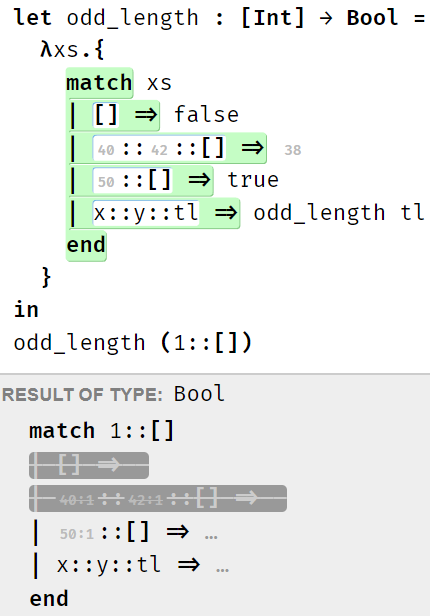
\includegraphics[scale=0.47]{imgs/pat_match_pat_holes.png}}%
	\subcaptionbox{Pattern matching with expression holes\label{fig:exp-hole}}{
		\raisebox{\dimexpr\ht2-\height}{
			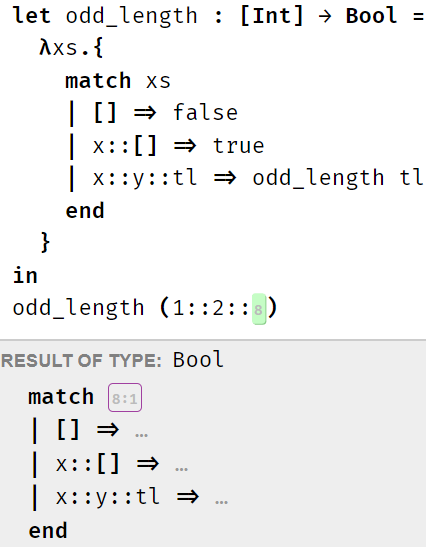
\includegraphics[scale=0.47,valign=t]{imgs/pat_match_exp_holes.png}
			\vphantom{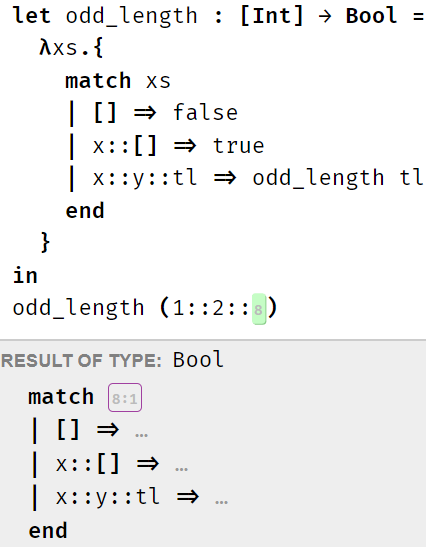
\includegraphics[scale=0.47,valign=t]{imgs/pat_match_exp_holes.png}}
		}
	}
	\hfil
	\subcaptionbox{Pattern matching with pattern holes\label{fig:pat-hole}}{
		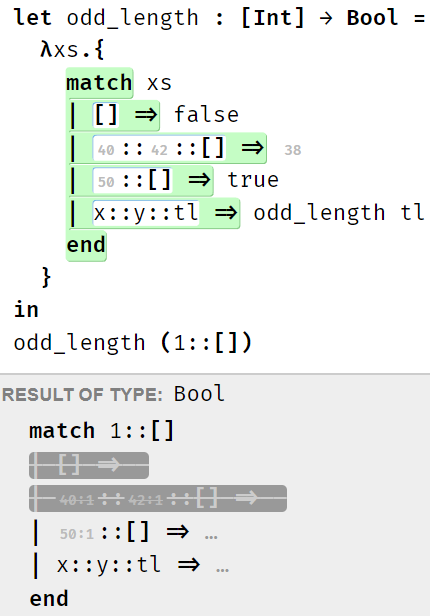
\includegraphics[scale=0.47,valign=t]{imgs/pat_match_pat_holes.png}
	}
	\caption{Live Evaluation with Expression and Pattern Holes}
	\label{fig:evaluation-ex}
\end{figure}


In \autoref{fig:exp-hole}, we apply the function \li{odd_length} to an argument that contains an expression hole with id \li{8}. Although the argument is indeterminate and cannot be fully-evaluated, per Hazel's live dynamic semantics, we substitute the partially evaluated argument into the function body and continue as far as possible. The argument then becomes the scrutinee of our \li{match} expression, and we proceed with pattern matching. Beginning with the first pattern, regardless of hole filling, the outermost constructor of our scrutinee is always a cons operator \li{::} rather than the empty list \li{[]}. Thus, our scrutinee must not match the first pattern \li{[]}, and we continue to the next rule. For the second pattern, our scrutinee always contains at least two elements while the pattern specifies only one element, so again, the expression must not match, and evaluation move to consider the third pattern. In this case, as the scrutineee indeed always contains at least two elements, the third match finally succeeds. Correspondingly, \li{x} is bound to \li{1}, \li{y} is bound to \li{2}, and \li{tl} is bound to the hole with id \li{8}. Evaluation then proceeds to the recursive call, and in this frame, our scrutinee becomes just an expression hole. Because we do not know whether the hole will be filled with an empty list or some other contents, we cannot determinately say whether it matches the pattern \li{[]}, hence evaluation must pause. We cannot proceed without further hole filling, so the entire \li{match} expression becomes indeterminate, displayed as the final result at the bottom of the image. Note that the scrutinee in the final result is indeed just the expression hole with id \li{8}.

In \autoref{fig:pat-hole}, our argument no longer contains any expression holes, but indeterminacy still arises due to the pattern holes in the second and third rules of the \li{match} expression. Specifically, evaluation begins by analyzing the scrutinee against the first pattern, and as \li{1 :: []} is not the empty list, we determine it must not match the first pattern. Likewise, despite the presence of pattern holes, the second pattern may only be matched by a two element list, so our scrutinee must not match it, and we continue to the third pattern. The third pattern gives the most interesting case. It indeed specifies a list with a single element, but the head of the pattern is a  pattern hole with id \li{50}, indicating that the first element of the scrutinee must match some yet-unknown pattern. If hole \li{50} were filled with the integer pattern \li{1} or a variable \li{x}, then \li{1::[]} would match. However, for many other hole fillings, e.g. the integer \li{2}, the match clearly fails. As a result, we can only state that \li{1::[]} indeterminately matches the third pattern, and evaluation must pause. Again, the entire \li{match} expression becomes indeterminate and is shown as the final result. By striking out the first two rules and displaying them in gray, we indicate to the user that evaluation has already proceeded past these cases.

\subsection{Exhaustiveness Checking with Pattern Holes}\label{sec:exhaustiveness}
With the dynamic semantics for live evaluation now clear, let us consider how to statically reason about this dynamic behavior through checks such as \emph{exhaustiveness analysis}. Recall that, in a language without holes, exhaustiveness requires that every expression of appropriate type matches at least one of the patterns in a \li{match} expression. When we introduce holes, however, exhaustiveness becomes more subtle, and we again must reason conservatively about all possible hole fillings and thereby handle cases of indeterminacy.

\begin{figure}
	\centering
	% Capture tallest image in box 3
	\setbox3=\hbox{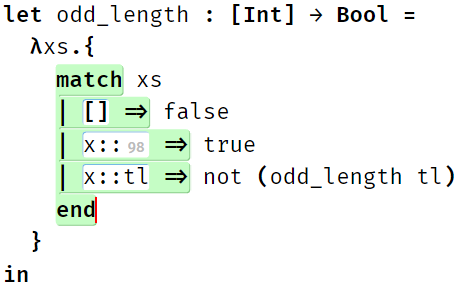
\includegraphics[scale=0.45]{imgs/exhaustive.png}}%
	\subcaptionbox{Indeterminately Exhaustive\label{fig:may-exhaustive}}{
		\raisebox{\dimexpr\ht3-\height}{
			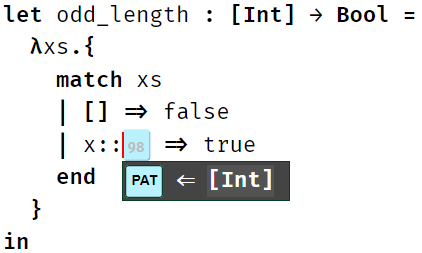
\includegraphics[scale=0.45,valign=t]{imgs/maybe_exhaustive.png}%
			\vphantom{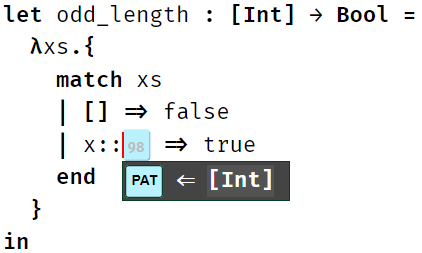
\includegraphics[scale=0.45,valign=t]{imgs/maybe_exhaustive.png}}
		}
	}
	\hfil
	\subcaptionbox{Necessarily Inexhaustive\label{fig:not-exhaustive}}{
		\raisebox{\dimexpr\ht3-\height}{
			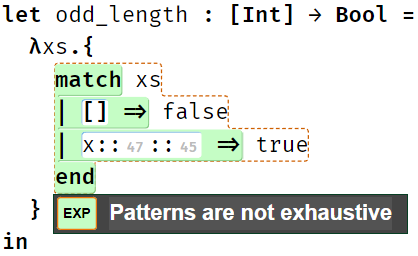
\includegraphics[scale=0.45,valign=t]{imgs/not_exhaustive.png}%
			\vphantom{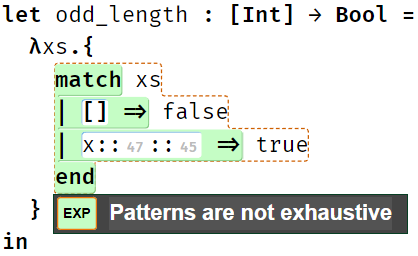
\includegraphics[scale=0.45,valign=t]{imgs/not_exhaustive.png}}
		}
	}
	\hfil
	\subcaptionbox{Necessarily Exhaustive\label{fig:must-exhaustive}}{
		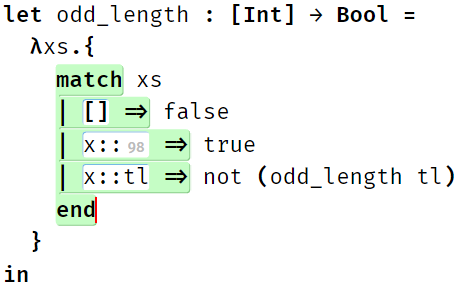
\includegraphics[scale=0.45,valign=t]{imgs/exhaustive.png}
	}
	\caption{Exhaustiveness Checking with Pattern Holes}
	\label{fig:exhaustiveness}
\end{figure}

Explicitly, assume the editor state is as in \autoref{fig:may-exhaustive}. The \li{match} expression contains two rules, the first with an empty list pattern \li{[]}, and the second with a cons cell pattern \li{::} with a variable \li{x} at the head and a pattern hole at the tail. The cursor is placed over the pattern hole, and Hazel is able to infer the type of the pattern as \li{[Int]} from the surrounding context, presenting this information to the user. Should we consider such an expression to be exhaustive? If the user fills the pattern hole with a variable \li{xs}, then the \li{match} is indeed exhaustive: any empty list matches the first pattern, and any non-empty list matches the second pattern. However, if the user instead fills the hole with, say, \li{[]} or \li{y::tl}, then a list with three elements would fail to match any pattern. Thus, without further hole-filling, we can only soundly state that the \li{match} is \emph{indeterminately exhaustive}.

While we cannot guarantee exhaustiveness in \autoref{fig:may-exhaustive}, such indeterminacy does not necessarily reflect an error on the user's part. Instead, they may simply be in the middle of on-going editing, working towards what will soon become an exhaustive expression. To avoid distracting the user with unnecessary information in such a case, in Hazel, we choose not to alert the user of indeterminate exhaustiveness. Instead, we only report an error when, regardless of hole fillings, the expression is always inexhaustive. We say such a \li{match} is \emph{necessarily inexhaustive}, and \autoref{fig:not-exhaustive} provides an illustrative example. The first given rule given only matches the empty list, and the second rule only possibly matches lists with at least two elements, with this holding regardless of the choice of hole-fillings. Thus, in any hole filling, a one element list such as \li{1 :: []} will not match any of the given patterns, and correspondingly, we display an error to the user. Note that the entire \li{match} expression is also resultingly placed within a non-empty hole. This is necessary to prevent evaluation from getting "stuck" when the scrutinee witnesses the inexhaustiveness.

Finally, even with the presence of pattern holes, there are still cases where we can in fact guarantee exhaustiveness. Considering \autoref{fig:must-exhaustive}, the first and third patterns together already cover all appropriately typed expressions. Thus, regardless of how the pattern hole in the second rule is filled, the \li{match} expression as a whole will always be exhaustive, i.e. it is \emph{necessarily exhaustive}. Note that we do not make a visual distinction between necessarily exhaustive and indeterminately exhaustive expressions, again because such information is more likely to be distracting than useful to the user. However, the semantic distinction is interesting to note, and it may be of use to future editor services designed around such holes. 

\subsection{Redundancy Checking with Pattern Holes}\label{sec:redundancy}
From a certain point of view, exhaustiveness checking guarantees a notion of \emph{sufficiency} - that the patterns in a \li{match} expression are sufficient to cover all possible values of the scrutinee's type. Redundancy checking, on the other hand, guarantees a notion of \emph{necessity} - that all the patterns in a \li{match} expressions are in fact required in that none is fully subsumed by other patterns earlier in the sequence. Explicitly, we say that a pattern $p$ in a \li{match} expression is redundant if, for every value $e$ of the scrutinee's type matching $p$, necessarily $e$ also matches some pattern $p^\prime$ preceding $p$ in the sequence of rules. Because a \li{match} expression considers rules one-by-one from the top down, a rule with a redundant pattern will be an unreachable code path. 

As the reader should now anticipate, including pattern holes again requires us to reason conservatively about all possible hole-fillings, thereby introducing indeterminacy into our analysis. That is, a pattern may be either \emph{necessarily redundant}, \emph{necessarily irredundant}, or \emph{indeterminately irredundant} due to the presence of expression or pattern holes. Similarly to how we handled exhaustiveness checking, we again only alert the user in cases where an error is guaranteed, i.e. when a rule is necessarily redundant.

\begin{figure}
	\centering
	\subcaptionbox{Necessarily Irredundant (first two patterns) + Indeterminately Irredundant (third pattern)\label{fig:may-redundant}}{
		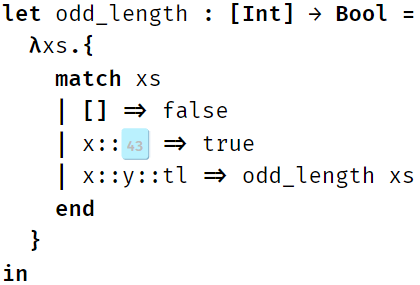
\includegraphics[scale=0.5,valign=t]{imgs/maybe_redundant.png}%
		\vphantom{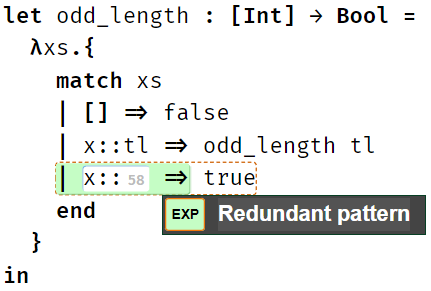
\includegraphics[scale=0.5,valign=t]{imgs/redundant.png}}
	} 
	\hfil
	\subcaptionbox{Necessarily Redundant (third pattern) \label{fig:must-redundant}}{
		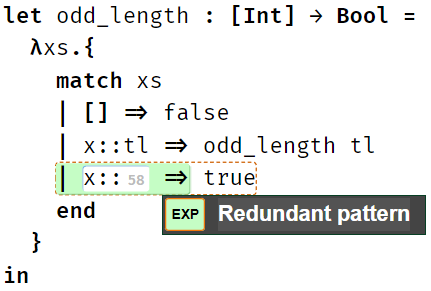
\includegraphics[scale=0.5,valign=t]{imgs/redundant.png}
	}%
	\caption{Redundancy Checking with Pattern Holes}
	\label{fig:redundancy}
\end{figure}

\autoref{fig:redundancy} concretely demonstrates all of these possibilities, continuing with our running example of an \li{odd_length} function. In the editor state in \autoref{fig:may-redundant}, there is a pattern hole in the second pattern. Depending on how this pattern hole is filled, the third pattern can be made either redundant or irredundant. Explicitly, if we filled the hole with the empty list \li{[]}, then the third pattern is the only one which matching lists with more than one element, so it is irredundant. If instead we filled the hole with \li{y::tl}, then the second pattern is in fact the same as third pattern, and obviously subsumes it. Thus, we can only soundly state that the third pattern is indeterminately irredundant.

For the second pattern itself, despite containing a pattern hole, we can still deem it necessarily irredundant. The only pattern proceeding it is an empty list \li{[]}, while the second pattern only matches non-empty lists regardless of hole filling. Thus, no hole filling allows the second pattern to be made redundant by the first. Note that, vacuously, the first pattern is also necessarily irredundant - it cannot be subsumed by previous rules because there are no previous rules. Similarly, the first pattern of any \li{match} expression is necessarily irredundant, except in the case when the scrutinee's type has no values at all (e.g. is of \li{void} type). In this case, all rules are necessarily redundant.

Finally, the editor state in \autoref{fig:must-redundant} showcases a necessarily redundant pattern. Explicitly, regardless of the choice of hole filling, the third pattern can only be matched by a non-empty list. However, the second pattern already matches all such non-empty lists. Thus, the third pattern is necessarily redundant, and correspondingly, we report an error to the user. Note that, in this particular case, the first two rules are already exhaustive, so any pattern we could possibly place in the third rule will be necessarily redundant. More generally, stating that a pattern $p$ is redundant is equivalent to stating that the preceding patterns exhaustively cover all values matching $p$. As we will explore in more detail in \autoref{sec:analyses}, this enables us to reduce the problem of redundancy checking to that of exhaustiveness checking.

\section{Mechanization}\label{sec:mechanization}
To round off our development, we also seek to ensure its correctness by proving various metatheoretical and semantic theorems. However, as discussed, pattern matching with holes in both expressions and patterns can be quite intricate, requiring reasoning about a three-valued logic of must, must not, and indeterminate judgments. Thus, even with on-paper proofs showing that such a system is correct, it can be difficult to have full confidence that all possibilities have been considered. Anecdotally, the current in-progress work on this system already contains some 150+ pages of tediously typed out proofs, and is likely to contain at least a few mistakes. To address this, we plan to mechanize the semantics and metatheory of our calculus in the Agda proof-assistant.

Briefly, Agda is a dependently typed functional programming language based on a variant of Martin-L\"of type theory known as the Unified Theory of Dependent Types \cite{DBLP:books/daglib/0078470, norell:thesis}. With dependent types, the division between types and values becomes blurry - types may be parameterized by arbitrary values, and types may be given as an argument or result of functions. Moreover, through the well-known Curry-Howard correspondence aka "types as propositions", a type $T$ may be considered as equivalent to the proposition "$T$ is inhabited". By designing appropriate datatypes, types may then encode mathematical statements, and constructing an Agda term of that type provides proof of the statement's correctness. Using this approach, we plan to verify all major theorems required to ensure our systems correctness.

%% Bibliography
\newpage
\bibliography{references.bib}

\end{document}
